\documentclass[11pt]{article}

\usepackage{amsmath, amsthm, amssymb, mathtools, commath}
\usepackage{datetime, geometry, xcolor, tcolorbox, graphicx, calc
	%enumitem
}
\usepackage[tikz]{mdframed}
\usepackage{tikz}

\geometry{
	right=0.5in,
	left=0.5in,
	top=1in,
	bottom=0.8in
}

\usepackage{fancyhdr}

\pagestyle{fancy}

\fancyhf{}
\lhead{Problem Set 1. Probability Basics}
\rhead{Vinesh Benny}
\rfoot{\thepage}

%\renewcommand{\headrulewidth}{0pt}

\title{STAB52 -- Problem Set 1. Probability Basics}
\author{Vinesh Benny}

\renewcommand\theenumii{\roman{enumii}}
\renewcommand\labelenumii{\theenumii}      %This changes the labelling for second level of enum globally. Should use enumitem instead.

\renewcommand{\qedsymbol}{$ \blacksquare $}

\definecolor{correct}{RGB}{37,150,190}

\mdfsetup{%
	middlelinecolor=blue!40,
	middlelinewidth=1pt,
	backgroundcolor=blue!25!purple!10!,
	roundcorner=5pt,
%	innerleftmargin=1cm,
%	innerrightmargin=1cm
}

%\usepackage{fourier}
\renewcommand{\rmdefault}{bch}
%\usepackage[sfdefault]{roboto}  %% Option 'sfdefault' only if the base font of the document is to be sans serif
%\usepackage[T1]{fontenc}
%\renewcommand{\familydefault}{\sfdefault}

%\pagecolor[rgb]{0,0,0} %black    % to change page to night mode
%\color[rgb]{0.5,0.5,0.5} %grey

\begin{document}
%	\maketitle
	\begin{enumerate}
		\item (Setting up sample spaces) Assume two standard six-sided dice are rolled one after the other.
			\begin{enumerate} % [label={\roman*}]
				\item Restrict attention to the first roll, and list all possible outcomes of this random experiment.
					\begin{mdframed}
						First roll can either be 1, 2, 3, 4, 5, or 6.  $\left( S =  \left\lbrace x \in \mathbb{N} \mid 1 \leq x \leq 6  \right\rbrace \right) $\\
						We do not care about the outcomes of the second roll.
					\end{mdframed}
				\item Now consider both rolls, and list the outcomes of the most general sample space you can define.
					\begin{mdframed}
						Each roll can either be 1, 2, 3, 4, 5, or 6. Therefore outcomes are: $ \left( S =  \left\lbrace x, y \in \mathbb{N} \mid 1 \leq x, y \leq 6  \right\rbrace \right) $ or\\
						\textbraceleft (1, 1), (1, 2), (1, 3), (1, 4), (1, 5), (1, 6),\\
						(2, 1), (2, 2), (2, 3), (2, 4), (2, 5), (2, 6),\\
						(3, 1), (3, 2), (3, 3), (3, 4), (3, 5), (3, 6),  \\
						(4, 1), (4, 2), (4, 3), (4, 4), (4, 5), (4, 6),  \\
						(5, 1), (5, 2), (5, 3), (5, 4), (5, 5), (5, 6),  \\
						(6, 1), (6, 2), (6, 3), (6, 4), (6, 5), (6, 6) \textbraceright
					\end{mdframed}
			\end{enumerate}

		\item (Set theory) Consider two arbitrary events $ A, B \in S $ and describe the following events using set operations.
			\begin{enumerate}
				\item Both events occur.
					\begin{mdframed}
						$ A \cap B $
					\end{mdframed}
				\item At least one event occurs.
					\begin{mdframed}
						$ A \cup B $
					\end{mdframed}
				\item Neither event occurs.
					\begin{mdframed}
						$ \neg \left( A \cup B \right)  $
					\end{mdframed}
				\item Only event $ A $ but not event $ B $ occurs, i.e. $ \left\lbrace s \in S : s \in A \text{ and } s \notin B \right\rbrace $.\\
				Note: this set operation is called \textit{difference} and is denoted A -- B (minus) or A\textbackslash B (back-slash).
					\begin{mdframed}
						$ A \cap \neg B $
					\end{mdframed}
				\item Exactly one event occurs.\\
				Note: this set operation is called \textit{symmetric difference} and is denoted by $ A\triangle B $. In logic it is also called \textit{exclusive OR} (XOR).
				\begin{mdframed}
					$ \left( A \cap \neg B \right) \cup \left( \neg A \cap B \right) $
				\end{mdframed}
			\end{enumerate}

		\newpage
		\item (Blitzstein: \S 1, Q42-43) For arbitrary events A, B use the probability axioms to show:\\
			{\footnotesize The definition of the difference ($ - $) and symmetric difference ($ \triangle $) set operations are given in problem 2.iv and 2.v.}
			\begin{enumerate}
				\item $ P(A - B)=P(A) - P(A \cap B) $.
					\begin{mdframed}
						\begin{proof}
							Recall: $ A = (A \cap B) \cup (A \cap B^c) = (A \cap B) \cup (A - B)$, where $ (A \cap B) $ and $ (A - B) $ are disjoint.\\
							$ \therefore P(A) = \underbrace{P(A \cap B) + P(A - B)}_{\text{By the additivity axiom.}} \implies  P(A - B)=P(A) - P(A \cap B ) \qedhere$
						\end{proof}
					\end{mdframed}
				\item $P(A \triangle B)=P(A)+P(B) - 2P(A \cap B) $.
					\begin{mdframed}
						\begin{proof}
							Recall: $ A - B $ and $ B - A $ are disjoint.
							\begin{align*}
								P(A \triangle B) &= P((A - B) \cup (B - A))\\
								&= P(A-B) + P(B-A) &\text{By the additivity axiom.}\\
								&= \left( P(A) - P(A \cap B) \right) + \left( P(B) - P(A \cap B) \right) &\text{By part i}\\
								\therefore &=P(A)+P(B) - 2P(A \cap B) &\qedhere
							\end{align*}
						\end{proof}
					\end{mdframed}
			\end{enumerate}

		\item Consider three arbitrary sets $ A, B, C $ represented by colored circles in the Venn diagram below.
			\begin{mdframed}[default, userdefinedwidth=4.8cm]
%				\resizebox{4cm}{!}{\begin{tikzpicture}
%					\definecolor{vennred}{HTML}{ff989b}
%					\definecolor{vennblue}{HTML}{90ccff}
%					\definecolor{venngreen}{HTML}{cbe196}
%					\begin{scope}[blend group = soft light]
%%						\fill[red!30!white!90]   ( 150:1.2) circle (2);
%						\fill[vennred]   ( 150:1.2) circle (2);
%%						\fill[blue!30!white!90] (270:1.2) circle (2);
%						\fill[vennblue] (270:1.2) circle (2);
%%						\fill[green!30!white!90]  (30:1.2) circle (2);
%						\fill[venngreen]  (30:1.2) circle (2);
%					\end{scope}
%					\node at (135:3.4) {$ A $};
%					\node at (45:3.4) {$ B $};
%					\node at (240:3.3)	{$ C $};
%					\node at ( 150:2)    {$ F $};
%					\node at (90:1.5) 	{$ G $};
%					\node at (210:1.5) 	{$ I $};
%					\node [] {$ H $};
%				\end{tikzpicture}}
				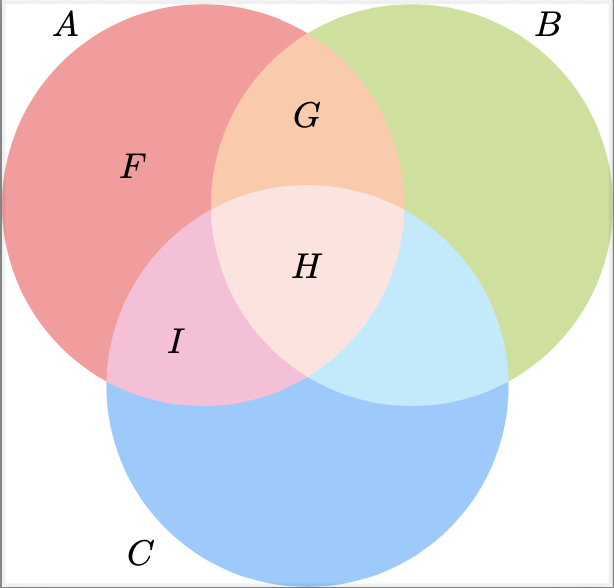
\includegraphics[width=4cm]{venn_pic.png}
			\end{mdframed}
			\begin{enumerate}
				\item Describe the strictly pink area $ F $ using set operations on $ A, B, C $.
					\begin{mdframed}
						$ F = A \cap \neg (B \cup C) $
					\end{mdframed}
				\item Describe the strictly brown area $ G $ using set operations on $ A, B, C $.
					\begin{mdframed}
						$ G = A \cap B \cap \neg C $
					\end{mdframed}
				\newpage
				\item Show that $ P(A \cup B \cup C)=P(A)+P(B)+P(C) - P(A \cap B) - P(B \cap C) - P(A \cap C)+ P (A \cap B \cap C ) $, i.e. prove the 3-set version of the inclusion-exclusion principle.
					\begin{mdframed}
						\begin{proof} By using the 2-set version of the inclusion principle, we can prove
							\begin{align*}
								P(A \cup B \cup C) &= P(A \cup (B \cup C))	\qquad\qquad\text{{\small Treating $ B \cup C $ as one event.}}\\
								&= \underbrace{P(A) + P(B \cup C) - P(A \cap (B \cup C))}_{\text{By 2-set version.}}\\
								&= P(A) + P(B \cup C) - P((A \cap B) \cup (A \cap C))\\
								&= P(A) + \underbrace{P(B) + P(C) - P(B \cap C)}_{\text{By 2-set version.}} - P((A \cap B) \cup (A \cap C))\\
								&= P(A) + P(B) + P(C) - P(B \cap C) - \underbrace{P(A \cap B) + P(A \cap C) - P(A \cap B \cap C)}_{\text{By 2-set version.}}\\
								&= P(A) + P(B) + P(C) - P(A \cap B) - P(A \cap C) - P(B \cap C) + P(A \cap B \cap C) \qedhere
							\end{align*}
						\end{proof}
					\end{mdframed}
			\end{enumerate}

		\item (Inclusion-exclusion principle; SOA Exam P, May 2003) A survey of a groups viewing habits over the last year revealed the following information:
			\begin{itemize}
				\begin{minipage}[t]{\widthof{14\% watched gymnastics and baseball $ (G \cap B)  $} + 1cm}
					\item 28\% watched gymnastics $ (G) $
					\item 19\% watched soccer $ (S) $
					\item 12\% watched baseball and soccer $ (B \cap S) $
					\item 8\% watched all three sports. ($ G \cap B \cap S) $
				\end{minipage}
				\begin{minipage}[t]{\widthof{10\% watched gymnastics and baseball $ (G \cap S) $}}
					\item 29\% watched baseball $ (B) $
					\item 14\% watched gymnastics and baseball $ (G \cap B)  $
					\item 10\% watched gymnastics and soccer $ (G \cap S) $
				\end{minipage}
			\end{itemize}
			Calculate the percentage of the group that:
				\begin{enumerate}
					\item Watched only gymnastics last year.
						\begin{mdframed}
							This is the same as watching gymnastics but not soccer or baseball. i.e. $ (G - (S \cup B)) $.
							\begin{align*}
								\left(G - \left(S \cup B\right)\right) &= \underbrace{\left(G - \left(G \cap \left(S \cup B\right) \right) \right)}_{\text{From 3i.}}\\
								&= G - \left( \left(G \cap S \right) \cup \left(G \cap B \right)   \right)\\
								&= G - \left( \left(G \cap S \right) + \left(G \cap B \right)  - \left(G \cap B \cap S \right) \right)\\
								&= 0.28 - \left( \left(0.10\right) + \left(0.14\right)  - \left(0.08\right) \right)\\
								&= \textbf{0.12}
							\end{align*}
						\end{mdframed}
					\item Watched none of the three sports last year.
						\begin{mdframed}
							This is the same is $ \neg (G \cup B \cup S) $
							\begin{align*}
								\neg (G \cup B \cup S) &= 1 - (G \cup B \cup S)\\
								&= 1 - {\left( G + B + S - \left(G \cap B \right) - \left(G \cap S \right) - \left(B \cap S \right)  + \left( G \cap B \cap S \right) \right)} \qquad\qquad\text{{\small From 4iii.}} \\
								&= 1 - \left( 0.28 + 0.29 + 0.19 - \left(0.14\right) - \left(0.10\right) - \left(0.12\right)  + \left(0.08\right) \right)\\
								&= 1 - 0.48\\
								&= \textbf{0.52}
							\end{align*}
						\end{mdframed}
				\end{enumerate}

		\item (Betting) Probabilities are often expressed as fractional odds in betting situations. To fix ideas, consider a random experiment (e.g. basketball match) and a specific event (e.g. Raptors win by more than 10 points). When you bet money on the event, the amounts you win ($ W $) or lose ($ L $) are determined by the \textit{odds}, which are usually quoted as the ratio $ W/L $. The odds work as follows: if you wager $ L $ and the event occurs, then you win $ W $ on top of your original $ L $. If you wager $ L $ and the event does not occur, then you lose the $ L $ you wagered. You can scale $ L $ up or down and $ W $ will change proportionately. Suppose the event at hand, call it $ A $, has probability $ P (A) = p $. If you gamble on it, on average you win $ p $ fraction of times and lose $ 1-p $ fraction of times. So you average net gain is $ pW - (1 - p) L $.
			\begin{enumerate}
				\item Find the implied fair probability of a bet based on its odds $ W/L $, i.e. find the value of $ p $ in terms of $ W $, $ L $ such that $ pW - (1 - p)L = 0 $
				\item Let $ A $ be some event with odds $ 3/1 $ and let its complement $ A^c $ have odds $ 1/1 $. Find the values of the implied probabilities $ P(A) = p$, $ P(A^c) = q $ based on the odds. Do these satisfy the probability axioms?
				\item Using the previous part’s odds, find a betting strategy that always generates a profit, no matter what the outcome. Your strategy should consist of two different amounts to wager simultaneously on events $ A $ and $ A^c $.\\
				Note: The situation where you make risk-free money in gambling/finance is called \emph{arbitrage}.
			\end{enumerate}

	\end{enumerate}
\end{document}